\documentclass[tikz,border=10pt]{standalone}

\begin{document}
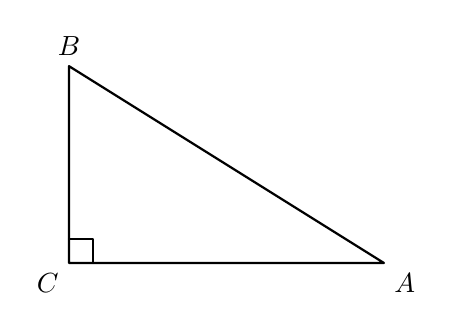
\begin{tikzpicture}[thick, line join=round, line cap=round]

    % --- 1. 定义几何顶点坐标 ---
    % 设定直角顶点 C 为原点 (0,0)
    % 假设 AC 长度为 4cm, BC 长度为 2.5cm
    \coordinate (C) at (0,0);
    \coordinate (A) at (4,0);
    \coordinate (B) at (0,2.5);

    % --- 2. 绘制三角形边界 ---
    \draw (A) -- (B) -- (C) -- cycle;

    % --- 3. 绘制直角符号 ---
    % 绘制在点 C 处的直角标志
    \draw (0,0.3) -- (0.3,0.3) -- (0.3,0);

    % --- 4. 标注顶点字母 ---
    % 使用 node 放置文本，其中 anchor 用于微调位置确保不遮挡线段
    \node [below right] at (A) {$A$};
    \node [above]       at (B) {$B$};
    \node [below left]  at (C) {$C$};



\end{tikzpicture}
\end{document}